\documentclass[tikz,border=2pt]{standalone}
\usepackage{amsmath,amssymb}
\usepackage{tikz}
\usetikzlibrary{matrix}

\begin{document}
% Project selection: one binary per project; every year's budget row sums only the
% expenditures of the selected (highlighted) projects.
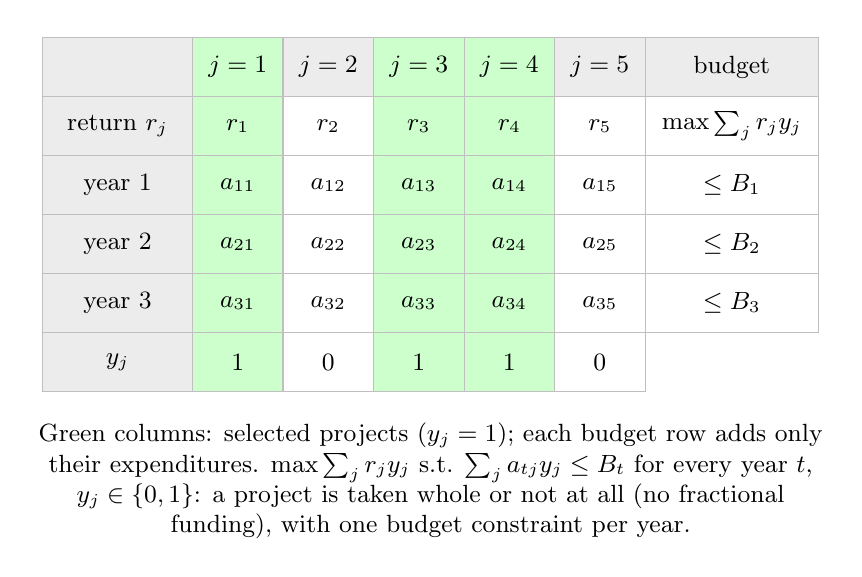
\begin{tikzpicture}[every node/.style={font=\small}]
	\matrix (T) [matrix of math nodes, nodes={minimum width=1.15cm, minimum height=7.5mm, anchor=center, draw=gray!50}, column 1/.style={nodes={minimum width=1.9cm}}, column 7/.style={nodes={minimum width=2.2cm}}, column sep=-\pgflinewidth, row sep=-\pgflinewidth] at (0,0) {
		|[fill=gray!15]| & |[fill=green!20]| j=1 & |[fill=gray!15]| j=2 & |[fill=green!20]| j=3 & |[fill=green!20]| j=4 & |[fill=gray!15]| j=5 & |[fill=gray!15]| \text{budget} \\
		|[fill=gray!15]| \text{return } r_j & |[fill=green!20]| r_1 & r_2 & |[fill=green!20]| r_3 & |[fill=green!20]| r_4 & r_5 & \max\sum_jr_jy_j \\
		|[fill=gray!15]| \text{year }1 & |[fill=green!20]| a_{11} & a_{12} & |[fill=green!20]| a_{13} & |[fill=green!20]| a_{14} & a_{15} & \le B_1 \\
		|[fill=gray!15]| \text{year }2 & |[fill=green!20]| a_{21} & a_{22} & |[fill=green!20]| a_{23} & |[fill=green!20]| a_{24} & a_{25} & \le B_2 \\
		|[fill=gray!15]| \text{year }3 & |[fill=green!20]| a_{31} & a_{32} & |[fill=green!20]| a_{33} & |[fill=green!20]| a_{34} & a_{35} & \le B_3 \\
		|[fill=gray!15]| y_j & |[fill=green!20]| 1 & 0 & |[fill=green!20]| 1 & |[fill=green!20]| 1 & 0 & \\
	};
	\node[anchor=north, align=flush center, text width=10cm] at ([yshift=-4pt]T.south) {Green columns: selected projects ($y_j=1$); each budget row adds only their expenditures. $\max\sum_jr_jy_j$ s.t. $\sum_ja_{tj}y_j\le B_t$ for every year $t$, $y_j\in\{0,1\}$: a project is taken whole or not at all (no fractional funding), with one budget constraint per year.};
\end{tikzpicture}
\end{document}
